
\section{UFOP - Laboratório iMobilis}
	\begin{frame}{Kit Odyssey}
        \vspace{-1em}
		\begin{multicols}{2}
				\begin{figure}[h]
					\centering
					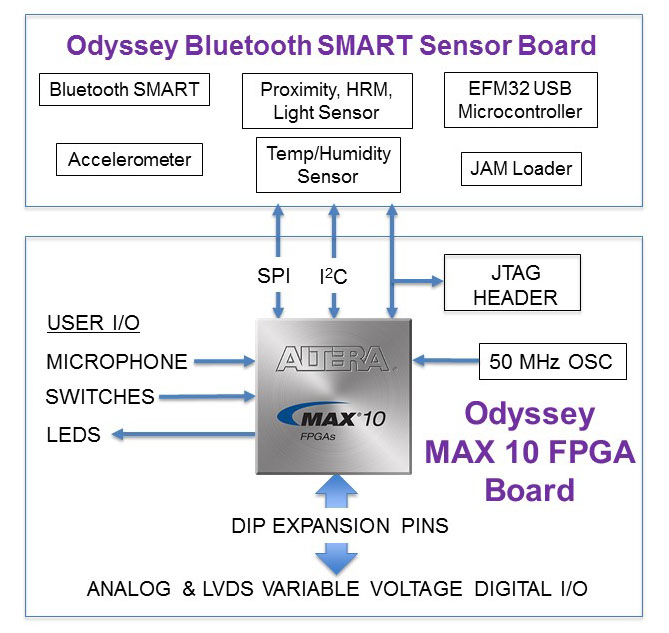
\includegraphics[width=0.48\textwidth]{img/imobilis/odyssey-esquematico.jpg}
					\caption{Esquemático do Odyssey IV.}
					\label{fig:odyssey-esquematico}
				\end{figure}
			\columnbreak
				\begin{itemize}
					\item Características:
					\begin{itemize}
						\setlength\itemsep{1em}
						\item Altera FPGA 10M08;
						\item 8 mil elementos lógicos
						\item 169 pinos;
						\item 55 nm.
					\end{itemize}
				\end{itemize}
		\end{multicols}
	\end{frame}

	\begin{frame}{Kit Odyssey}
		\begin{figure}[h]
			\centering
			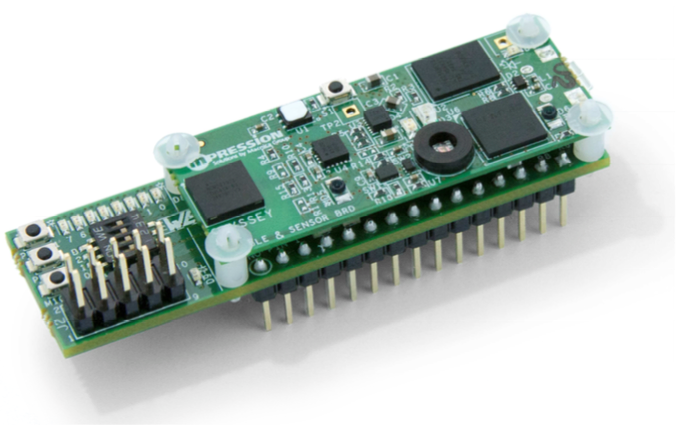
\includegraphics[width=0.7\textwidth]{img/imobilis/odyssey-foto.png}
			\caption{Odyssey IV.}
			\label{fig:odyssey-foto}
		\end{figure}
	\end{frame}


	\begin{frame}{Kit Mercurio IV}
        \vspace{-1em}
		\begin{itemize}
			\item Modelo EP4CE30F23 responsável possui cerca de $ 30 $ mil elementos lógicos, com $ 484 $ pinos de entrada e saída e utiliza \textit{clock} de $50Mhz$.
		\end{itemize}

		\begin{figure}[h]
			\centering
			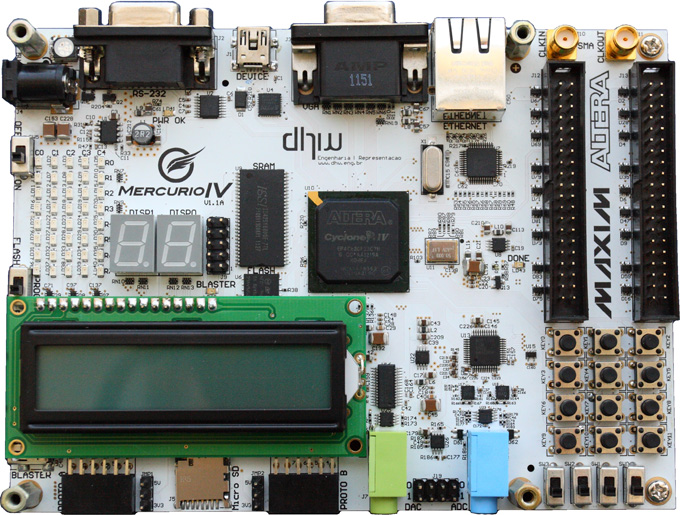
\includegraphics[width=0.55\textwidth]{img/imobilis/mercurio-foto.jpg}
			\caption{Mercurio IV.}
			\label{fig:mercurio-foto}
		\end{figure}
	\end{frame}

	\begin{frame}%{Kit Mercurio IV}
        \vspace{-1em}
		\begin{figure}[h]
			\centering
			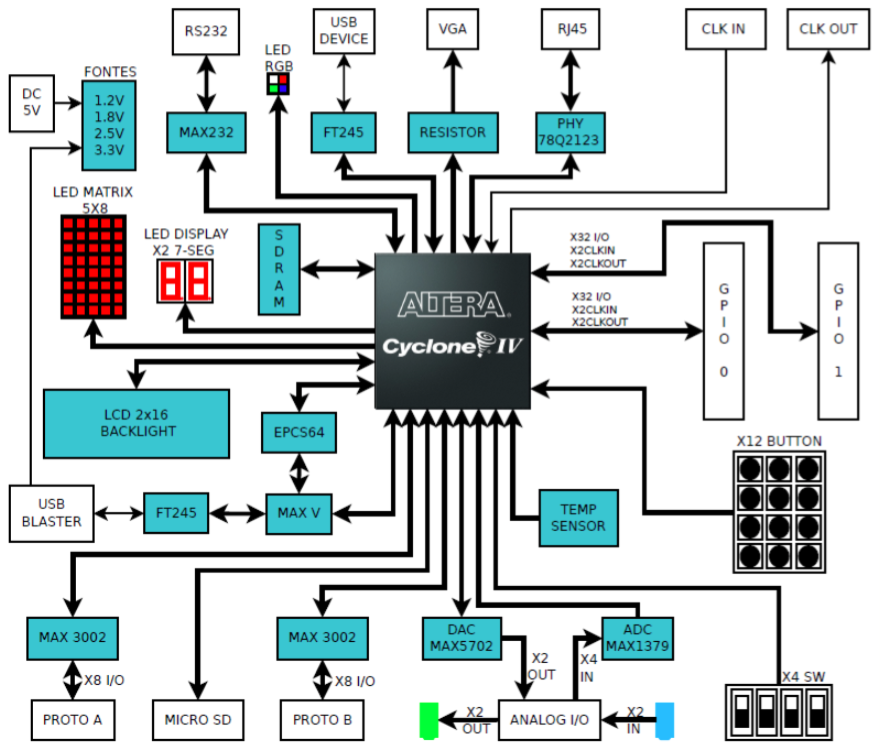
\includegraphics[width=0.68\textwidth]{img/imobilis/mercurio-esquematico.png}
			\caption{Pespectiva Geral dos Componentes do Mercurio IV.}
			\label{fig:mercurio-esquematico}
		\end{figure}
	\end{frame}


	\begin{frame}{Kit Helio Cyclone V}
		\begin{itemize}
			\setlength\itemsep{1em}
			\item Fabricado em tecnologia de silício de 28nm.

			\item Este FPGA integra num único dispositivo um sistema em \textit{hardware} baseado no processador ARM Cortex A9 dual-core e mais um grande conjunto de periféricos.

			\item Características:
			\begin{itemize}
				\setlength\itemsep{0.4em}
				\item Altera Cyclone V SoC -- 5CSXFC6C6U23C8NES / 5CSXFC5C6U23C7N
				\item HSMC expansion connector
				\item DDR3-SDRAM
				\item Micro SD Card
				\item Interfaces: 1Gb Ethernet, USB OTG, UART...
				\item Yocto Linux BSP
			\end{itemize}
		\end{itemize}
	\end{frame}

	\begin{frame}{Kit Helio Cyclone V}
        \vspace{-1em}
		\begin{figure}[h]
			\centering
			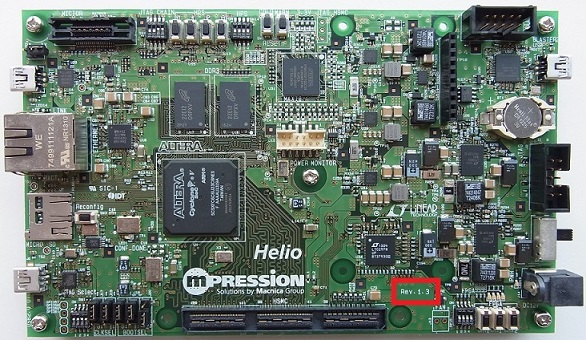
\includegraphics[width=0.8\textwidth]{img/imobilis/helio-foto.jpg}
			\caption{Componentes do Helio Cyclone V.}
			\label{fig:helio-foto}
		\end{figure}
	\end{frame}

	\begin{frame}%{Kit Helio Cyclone V}
        \vspace{-0.5em}
		\begin{figure}[h]
			\centering
			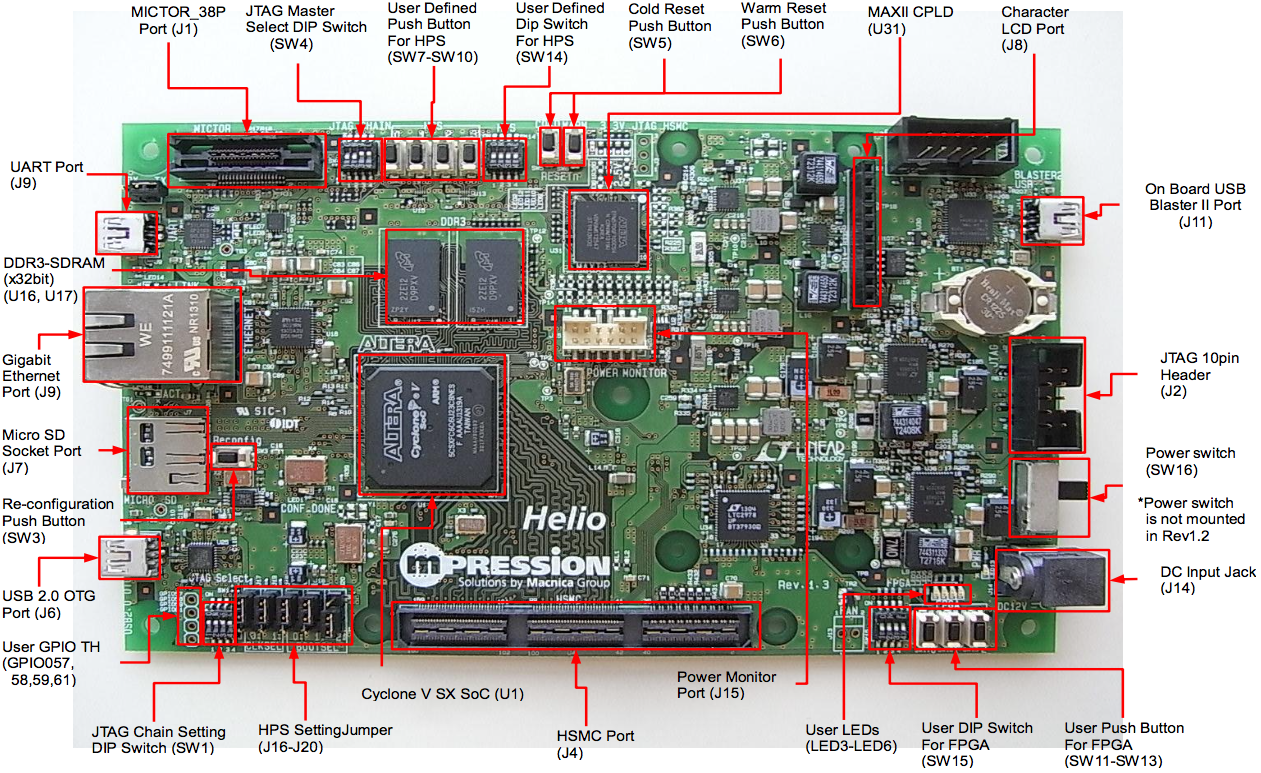
\includegraphics[width=0.95\textwidth]{img/imobilis/helio-foto-2.png}
			\caption{Componentes do Helio Cyclone V.}
			\label{fig:helio-foto2}
		\end{figure}
	\end{frame}

	\begin{frame}%{Kit Helio Cyclone V}
		\begin{figure}[h]
			\centering
			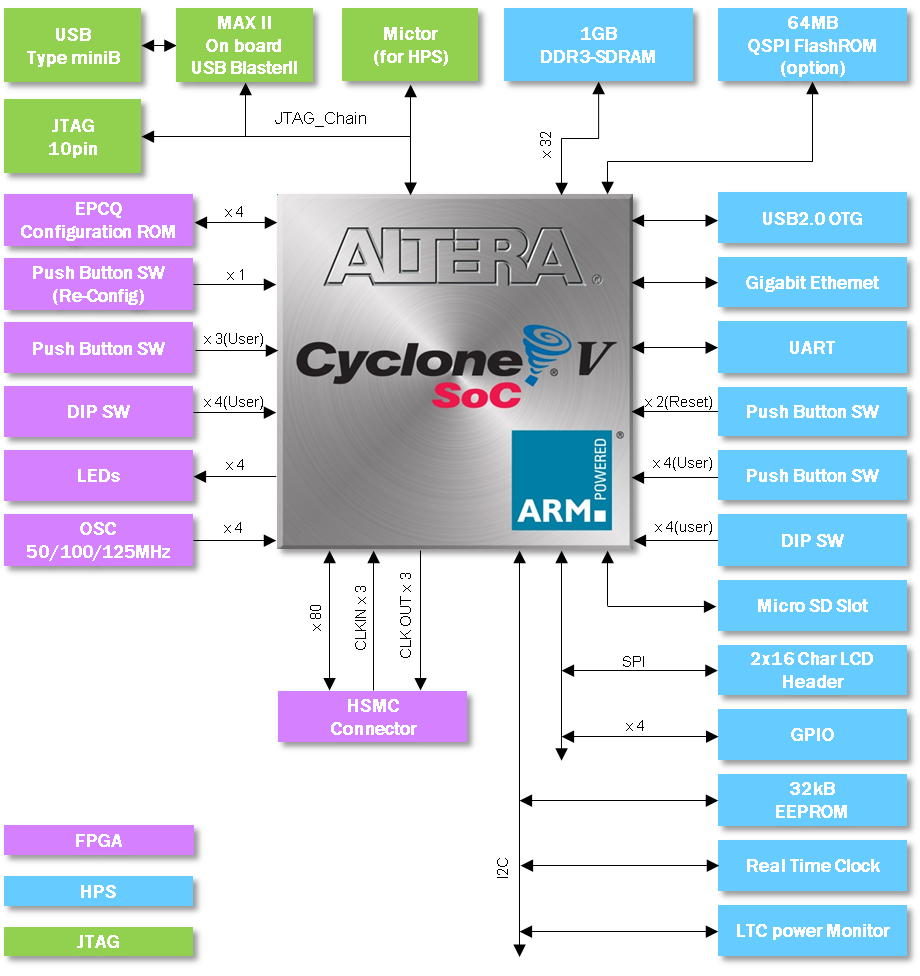
\includegraphics[width=0.53\textwidth]{img/imobilis/helio-esquematico.png}
			\caption{Esquemático do Helio Cyclone V.}
			\label{fig:helio-esquematico}
		\end{figure}
	\end{frame}



    \begin{frame}{Digilent Arty}
    \vspace{-0.5em}
        \begin{figure}[h]
            \centering
            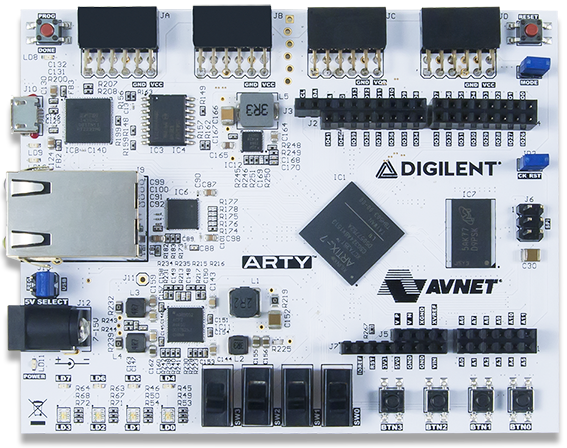
\includegraphics[width=0.6\textwidth]{img/imobilis/arty1.png}
            \caption{Componentes do Helio Cyclone V.}
            \label{fig:arty1}
        \end{figure}
    \end{frame}
    
    \begin{frame}%{Kit Helio Cyclone V}
        \begin{figure}[h]
        \centering
        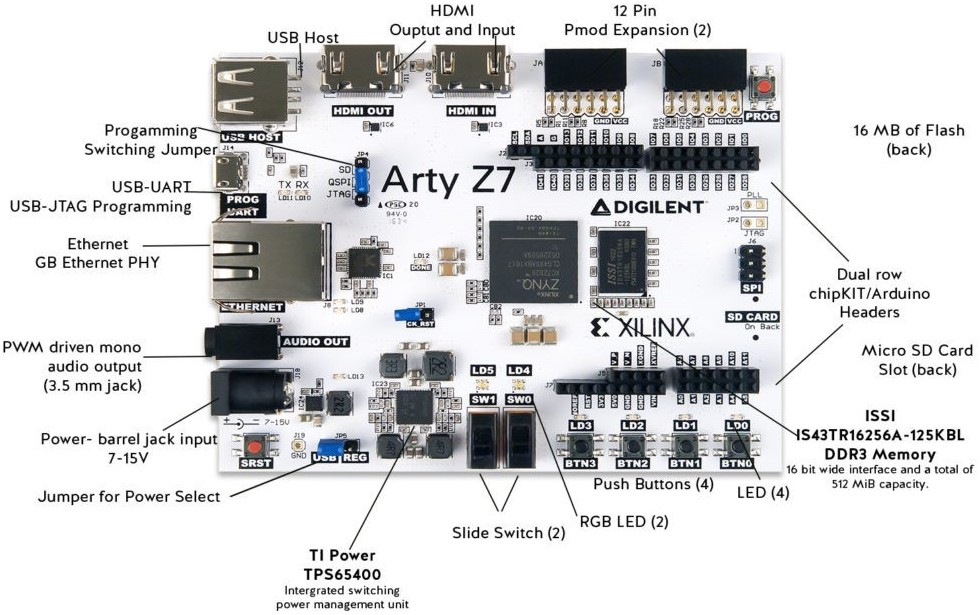
\includegraphics[width=0.9\textwidth]{img/imobilis/arty2.jpg}
        \caption{Esquemático do Arty.}
        \label{fig:arty2}
        \end{figure}
    \end{frame}

    \begin{frame}%{Kit Helio Cyclone V}
        \begin{figure}[h]
        \centering
        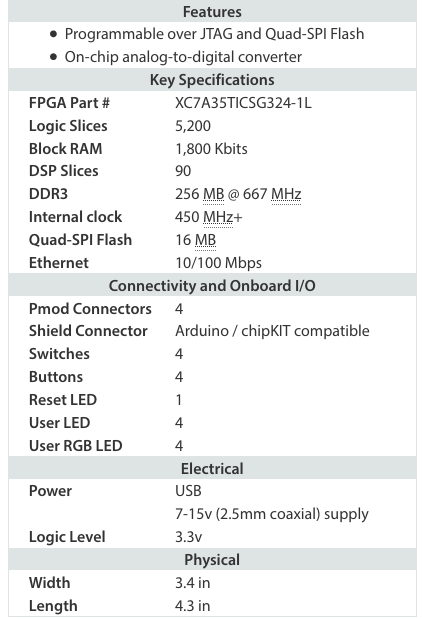
\includegraphics[width=0.37\textwidth]{img/imobilis/arty3.png}
        \caption{Esquemático do Helio Cyclone V.}
        \label{fig:arty3}
        \end{figure}
    \end{frame}



    \begin{frame}{Papilio Platform}
        \begin{figure}[h]
            \centering
            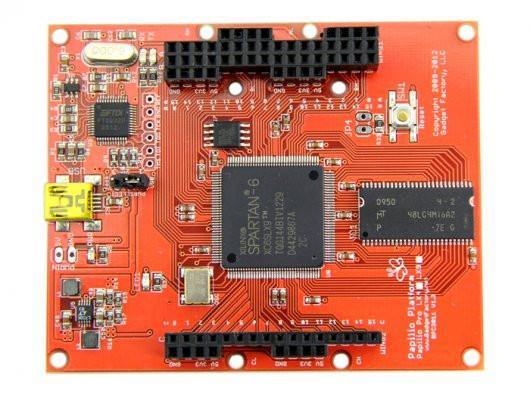
\includegraphics[width=0.6\textwidth]{img/imobilis/papilio.jpeg}
            \caption{Esquemático do Papilio Platform.}
            \label{fig:papilio}
        \end{figure}
    \end{frame}